\documentclass[11pt]{article}
\usepackage{homework}

\classname{361}
\homeworknum{4}



\begin{document}

% Environments

\newcommand{\state}[2]{\begin{statement}{#1} #2 \end{statement}}
\newcommand{\prob}[2]{\begin{problem}{#1} #2 \end{problem}}
\newcommand{\subprob}[1]{\begin{subproblem} #1 \end{subproblem}}
\newcommand{\sol}[1]{\begin{solution} #1 \end{solution}}
\newcommand{\fig}[2]{\begin{figure} \centering #2  \label{#1} \end{figure}}

\newcommand{\makebib}{
	\vfill
	\color{black}
	\nocite{*}
	\bibliography{references}{}
	\bibliographystyle{lucas_unsrt}
}
	

% Implication

\newcommand{\qwhere}{\quad \text{where} \quad}
\newcommand{\qimplies}{\quad \implies \quad}
\newcommand{\impliesq}{\implies \quad}



% Brackets

\newcommand{\paren}[1]{\left( #1 \right)}
\newcommand{\brac}[1]{\left[ #1 \right]}
\newcommand{\curly}[1]{\left\{ #1 \right\}}


% Greek

\newcommand{\alp}{\alpha}
\newcommand{\bet}{\beta}
\newcommand{\gam}{\gamma}
\newcommand{\del}{\delta}
\newcommand{\eps}{\epsilon}
\newcommand{\zet}{\zeta}
\newcommand{\tht}{\theta}
\newcommand{\kap}{\kappa}
\newcommand{\lam}{\lambda}
\newcommand{\sig}{\sigma}
\newcommand{\ups}{\upsilon}
\newcommand{\omg}{\omega}

\newcommand{\Gam}{\Gamma}
\newcommand{\Del}{\Delta}
\newcommand{\Tht}{\Theta}
\newcommand{\Lam}{\Lambda}
\newcommand{\Sig}{\Sigma}
\newcommand{\Omg}{\Omega}


% Text

\newcommand{\where}{\text{where }}

% Problem 1

\newcommand{\Hint}{H_\text{int}}
\newcommand{\ddcx}{\dd[3]{x}}
\newcommand{\psib}{\bar{\psi}}

\newcommand{\mh}{m_h}
\newcommand{\mmu}{m_\mu}
\newcommand{\me}{m_e}
\newcommand{\ma}{m_a}

\newcommand{\aexpt}{a_\text{expt.}}
\newcommand{\aQED}{a_\text{QED}}
\renewcommand{\GeV}{\giga\electronvolt}

\newcommand{\gamt}{\gam^5}

\state{Spin-wave theory~(P\&S 11.1)}{\hfix}

\prob{ \label{1a}
	Prove the following wonderful formula: Let $\phix$ be a free scalar field with propagator $\ev{T \phix \phio} = \Dx$.  Then
	\eqn{show1}{
		\ev{ T e^{i \phix} e^{-i \phio} } = e^{[ \Dx - \Do ]}.
	}
	(The  factor $\Do$ gives a formally divergent adjustment of the overall normalization.)
}

\sol{
	According to P\&S~(9.18),
	\eq{
		\ev*{T \phi(\xq) \phi(\xw)}{\Omg} = \frac{\int \DDphi \phi(\xq) \phi(\xw) \exp[ i \int \ddqx \cL ]}{\int \DDphi \exp[ i \int \ddqx \cL ]}.
	}
	We use this expression to write the left-hand side of Eq.~\refeq{show1}:
	\eqn{thing1}{
		\ev{ T e^{i \phix} e^{-i \phio} } = \frac{\int \DDphi e^{i \phix} e^{-i \phio} \exp[ i \int \ddqy \cL ]}{\int \DDphi \exp[ i \int \ddqy \cL ]}
		= \frac{\int \DDphi \exp[i \phix - i \phio + i \int \ddqy \cL ]}{\int \DDphi \exp[ i \int \ddqy \cL ]}.
	}
	For a free Klein-Gordon~(i.e., scalar) field, Eq.~(9.39) tells us that the generating functional $\ZJ$ is given by
	\eq{
		\ZJ = \Zo \exp[ -\frac{1}{2} \int \ddqx \ddqy \Jx \DF(x - y) \Jy ],
	}
	where $\Zo = Z[0]$.  Thus, we want to find some $\Jy$ such that
	\eqn{thing1b}{
		\ev{ T e^{i \phix} e^{-i \phio} } = \frac{\ZJ}{\Zo}
	}
	where in general
	\eq{
		\ZJ = \int \DDphi \exp[ i \int \ddqx [ \cL + \Jx \phi(x) ] ]
	}
	by (9.34).  Inspecting Eq.~\refeq{thing1}, we recognize the denominator as $\Zo$ and see that if
	\eq{
		\Jy = \delq(y - x) - \delq(y)
	}
	we have an expression like Eq.~\refeq{thing1b}.  Collecting these findings, we have
	\al{
		\ans{ \ev{ T e^{i \phix} e^{-i \phio} } }&= \frac{\ZJ}{\Zo} \\
		&= \exp[ -\frac{1}{2} \int \ddqy \ddqz \Jy \DF(y - z) \Jz ] \\
		&= \exp[ -\frac{1}{2} \int \ddqy \ddqz \Jy \DF(y - z) [ \delq(z - x) - \delq(z) ] ] \\
		&= \exp[ -\frac{1}{2} \int \ddqy [ \delq(y - x) - \delq(y) ] [ \DF(y - x) - \DF(y) ] ] \\
		&= \exp[ -\frac{1}{2} [ \DF(0) - \DF(x) - \DF(-x) + \DF(0) ] ] \\
		&= \exp[ \DF(x) - \DF(0) ] \\
		&\ans{\; = e^{[ \Dx - \Do ]}, }
	}
	as we wanted to show. \qed
}



\prob{ \label{1b}
	We can use this formula in Euclidean field theory to discuss correlation functions in a theory with spontaneously broken symmetry for $T < \TC$.  Let us consider only the simplest case of a broken $O(2)$ or $U(1)$ symmetry.  We can write the local spin density as a complex variable
	\eq{
		\sx = \sqx + i \swx.
	}
	The global symmetry is the transformation
	\eq{
		\sx \to e^{-i \alp} \sx.
	}
	If we assume that the physics freezes the modulus of $\sx$, we can parameterize
	\eqn{sx}{
		\sx = A e^{i \phix}
	}
	and write an effective Lagrangian for the field $\phix$.  The symmetry of the theory becomes the translation symmetry
	\eqn{symmetry}{
		\phix \to \phix - \alp.
	}
	Show that (for $d > 0$) the most general renormalizable Lagrangian consistent with this symmetry is the free field theory
	\eqn{show1b}{
		\cL = \frac{1}{2} \rho(\vgrad \phi)^2.
	}
	In statistical mechanics, the constant $\rho$ is called the \emph{spin wave modulus}.  A reasonable hypothesis for $\rho$ is that it is finite for $T < \TC$ and tends to 0 as $T \to \TC$ from below.
}

\sol{
	In accordance with the Klein-Gordon Lagrangian in P\&S~(2.6),
	\eqn{KGL}{
		\cL_\text{K-G} = \frac{1}{2} (\pt \phi)^2 - \frac{1}{2} m^2 \phi^2,
	}
	we interpret $(\vgrad \phi)^2$ as $(\pt \phi)^2$.
	
	The Lagrangian cannot have terms of $\order{\phi^n}$ for any $n \neq 0$ since $\phi(x)$ is not invariant under Eq.~\refeq{symmetry}.  Any combination of derivatives of $\phi$ is invariant, however, since $\alp$ is a constant and does not contribute to any derivative.  Thus, only terms like $\pt^n \phi^m$ (where $n$ denotes a power of $\pt$) for $n, m > 0$ and $n \geq m$ are consistent with the symmetry of Eq.~\refeq{symmetry} for $d$ an integer.
	
	Now we must determine which of these terms are renormalizable.  We know that the Lagrangian must have dimension $d$, and that $\phi$ has dimension $(d - 2) / 2$.  Taking a derivative adds a mass dimension.  The theory is renormalizable if the coupling constant $\rho$ has dimension greater than or equal to 0~\cite[p.~322]{Peskin}.  Let $p$ be the dimension of $\rho$.  The dimension of our allowed term is then
	\eq{
		[ \rho \pt^n \phi^m ] = p + n + m \frac{d - 2}{2},
	}
	which we require to be equal to $d$.  Thus we seek solutions to the system of equations
	\al{
		d &= p + n + m \frac{d - 2}{2}, &
		n &\geq m, &
		p &\geq 0.
	}
	Solving with Mathematica, we find that this system has two solutions: $n = m = 2$ and $p = 0$; and $n = m = 1$ and $p = d / 2$.  However, the term $\pt \phi$ for $n = m = 1$ does not contribute to the action because it is a total derivative and does not contribute when the integral over $\cL$ is evaluated:
	\eq{
		\int \dd[d]{x} \pt\phi = \phi \bigg|_{-\infty}^\infty
		= 0.
	}
	Thus the only possibility is $n = m = 2$.  Note that
	\eq{
		\pt^2 \phi^2 = \pt(\pt \phi^2)
		= 2 \pt( \phi \pt \phi)
		= \pt \phi \pt \phi + \phi \pt^2 \phi
		= (\pt \phi)^2,
	}
	since $\phi \pt^2 \phi$ is not invariant under Eq.~\refeq{sx}.  This means that $\rho$ must be dimensionless and that the only allowed terms in the Lagrangian are proportional to $(\pt \phi)^2$, which is consistent with Eq.~\refeq{show1b}. \qed
}



\prob{
	Compute the correlation function $\ev{ \sx \sao }$.  Adjust $A$ to give a physically sensible normalization (assuming that the system has a physical cutoff at the scale of one atomic spacing) and display the dependence of this correlation function on $x$ for $d = 1, 2, 3, 4$.  Explain the significance of your results.
}

\sol{
	Applying Eq.~\refeq{sx},
	\eq{
		\ev{ \sx \sao } = \ev*{ A e^{i \phix} \As e^{-i \phio} }
		= \ev*{ \abs{A}^2 } \ev*{ e^{i \phix} e^{-i \phio} }.
	}
	Now we can apply Eq.~\refeq{show1} to find
	\eqn{thing1c}{
		\ans{ \ev{ \sx \sao } = \abs{A}^2 \exp[ D(x) - D(0) ], }
	}
	where $D(x - y)$ is a Green's function.  Since our Lagrangian is similar to the Klein-Gordon Lagrangian Eq.~\refeq{2.6}, our Green's function is similar to that of the Klein-Gordon operator, which is given by P\&S~(2.56):
	\eq{
		(\pt^2 + m^2) D(x - y) = -i \delq(x - y).
	}
	The Feynman prescription for this Green's function is given by (2.59),
	\eqn{DF}{
		\DF(x - y) = \int \ddqpf \frac{i}{p^2 - m^2 + i \eps} e^{-i p \cdot (x - y)}.
	}
	For the Lagrangian in Eq.~\refeq{show1b}, we set $m = 0$ and insert a factor of $\rho$:
	\eq{
		\rho \pt^2 D(x - y) = -i \deld(x - y),
	}
	so adapting Eq.~\refeq{DF} for this situation yields
	\eqn{DF}{
		\DF(x - y) = \frac{1}{\rho} \int \dddpf \frac{i}{p^2 + i \eps} e^{-i p \cdot (x - y)}.
	}
	We see that $\DF(0)$ diverges, so we absorb it into the constant to make the normalization physically sensible.  We can do this because, as we showed in \ref{1b}, the theory is renormalizable.  Define $A'$ such that
	\eq{
		{A'}^2 = \abs{A}^2 e^{-D(0)}.
	}
	Then Eq.~\refeq{thing1c} can be written
	\eq{
		\ans{ \ev{ \sx \sao } =  {A'}^2 e^{D(x)}. }
	}
	
	To evaluate the divergent integral $D(x)$, we look to the Feynman parameter method we have been using to solve divergent integrals.  Apparently, the Schwinger parametrization is useful in deriving the Feynman parametrization, and it is given by~\cite{Feynman}
	\eq{
		\frac{1}{A} = \intoi \dds e^{-s A}.
	}
	Using this equation, we can write Eq.~\refeq{DF} as
	\eq{
		\DF(x) = \frac{1}{\rho} \int \dddpf \frac{i}{p^2} e^{-i p \cdot x}
		= \frac{i}{\rho} \int \dddpf \intoi \dds e^{-s p^2} e^{-i p \cdot x}.
	}
	Now we can complete the square in the exponential to get a Gaussian integral:
	\al{
		\DF(x) &= \frac{i}{\rho} \int \dddpf \intoi \dds \exp[ -s p^2 - i p \cdot x + \frac{x^2}{4 s} - \frac{x^2}{4 s} ] \\
		&= \frac{i}{\rho} \int \dddpf \intoi \dds \exp[ -s \paren{ p + \frac{i x}{2 s} }^2 - \frac{x^2}{4 s} ] \\
		&= \frac{i}{\rho (2 \pi)^d} \intoi \dds e^{-x^2 / 4 s} \int \dd[d]{u} e^{-s u^2} \\
		&= \frac{i}{\rho (2 \pi)^{d}} \intoi \dds e^{-x^2 / 4 s} \sqrt{ \frac{(2\pi)^d}{(2s)^d} } \\
		&= \frac{i}{\rho (4 \pi)^{d / 2}} \intoi \dds \frac{e^{-x^2 / 4 s}}{s^{d / 2}}
	}
	where we have used~\cite{QFT}
	\eq{
		\int \exp( -\frac{1}{2} x \cdot A \cdot x ) \dd[n]{x} = \sqrt{\frac{(2\pi)^n}{\det A}},
	}
	with $A$ a $d \times d$ diagonal matrix $2s$.  Using Mathematica to integrate with respect to $s$, we find
	\eq{
		\DF(x) = \frac{i}{\rho (4 \pi)^{d / 2}} \frac{2^{d - 2}}{x^{d - 2}} \Gam(d / 2 - 1)
		= \frac{i}{4 \pi^d \rho} \Gam(d / 2 - 1) x^{2 - d}.
	}
	The gamma function diverges as $d \to 2$, so as we have done in previous problems, we expand about $\eps = 2 - d$.  Evaluating the series expansion using Mathematica, we obtain
	\eq{
		\DF(x) = \frac{i}{4 \pi^{1 - \eps} \rho} \Gam(\eps / 2) x^\eps
		\approx \frac{i}{4 \pi \rho} \paren{ \frac{2}{\eps} - \gam + 2 \ln(\pi x) }
		\sim \frac{i}{2 \pi \rho} \ln(x)
		= i \ln(\frac{1}{x^{2 \pi \rho}}).
	}
	We Wick rotate $x \to i x$.  Then the dependence of the correlation function on $x$ for $d = 1, 2, 3, 4$ is
	\ans{\al{
		(d = 1) &\qquad \ev{ \sx \sao } \sim e^{-x / 2 \sqrt{\pi} \rho}, &
		(d = 2) &\qquad \ev{ \sx \sao } \sim x^{2 \pi \rho}, \\
		(d = 3) &\qquad \ev{ \sx \sao } \sim \frac{1}{x}, &
		(d = 4) &\qquad \ev{ \sx \sao } \sim \frac{1}{x^2}.
	}}%
	In $d > 2$ dimensions, the expectation value of the correlation function tends to 0 at large distances $x$.  For $d > 2$, it drops off more quickly as $d$ increases.  The $d \leq 2$ cases depend on $\rho$, which we assume is positive.  The $d = 1$ case drops off with increasing distance, and more quickly with smaller $\rho$.  For $d = 2$, the expectation value of the correlation function increases with increasing distance, and it blows up more quickly with larger $\rho$.
	
	These results are consistent with the Mermin--Wagner theorem, which states that a continuous symmetry cannot be broken in $d \leq 2$ dimensions~\cite{CMW}.  That is, in $d \leq 2$ dimensions, a symmetry-breaking field cannot have a nonzero vacuum expectation value~\cite[p.~460]{Peskin}.  A physical explanation is that each spin has more nearest neighbors in higher dimensions.  Since the spins are inclined to align with their neighbors, there is a higher degree of correlation in higher dimensions at the same distance.  In two dimensions, the correlations are weak enough that they are overpowered by the field fluctuations.
}






\state{Landau theory of phase transitions}{
	A ferroelectric crystal is one that supports a macroscopic polarization $P$, which usually arises because the underlying crystal structure does not have inversion symmetry.  However, as temperature or pressure is changed, the crystal may recover the inversion symmetry.  This can be modeled by Landau's theory of second order phase transitions, where we postulate a form for the free energy density (per unit volume)
	\eqn{given2}{
		\cF = \frac{a}{2} P^2 + \frac{b}{4} P^4 + \frac{c}{6} P^6 + \cdots,
	}
	where the coefficient $a = \ao (T - \Tc)$ is temperature dependent and all the other coefficients are constant.  Although the polarization $P$ is of course a vector, we assume that it can point only in a symmetry direction of the crystal, and so it is replaced by a scalar.
}

\prob{
	Assume that $b > 0$ and $c = 0$.  Use Eq.~\refeq{given2} to determine the form for the equilibrium $\PT$.
}

\sol{
	When $b > 0$ and $c = 0$, Eq.~\refeq{given2} becomes
	\eq{
		\cF = \frac{a}{2} P^2 + \frac{b}{4} P^4.
	}
	The equilibrium $\PT$ occurs at the minima of $\cF$, where $\dv*{\cF}{P} = 0$~\cite{Ferroelectricity}:
	\eq{
		\dv{\cF}{P} = a P + b P^3 = 0.
	}
	This implies
	\al{
		P &= 0, &
		P &= \pm \sqrt{-\frac{a}{b}}.
	}
	Note, however, that $P = 0$ is a local maximum of $\cF$:
	\eq{
		\left. \dv[2]{\cF}{P} \right|_{P = 0} = \brac{ a + 2 b P^2 }_{P = 0}
		= \ao (T - \Tc)
		< 0 \quad \text{when } T < \Tc,
	}
	which is the regime we are interested in for a ferroelectric~\cite[p.~556]{Ashcroft}\cite{Ferroelectricity}.  Thus the equiliibrium $\PT$ is given by
	\eq{
		\ans{ \PT = \pm \sqrt{\frac{\ao}{b} (\Tc - T)}. }
	}
	\vfix
}



\prob{ \label{2c}
	Including in $\cF$ the energy of the polarization coupled to an external electric field $E$, determine the dielectric susceptibility $\chi = \dv*{P}{E}$ both above and below the critical temperature.
}



\prob{
	Sketch curves for $\PT$, $\chiinvT$, and $\chiT$.
}



\prob{
	In a different material, the free energy is described by a similar form to Eq.~\refeq{given2}, but with $b < 0$ and $c > 0$.  By sketching $\cF$ at different temperatures, discuss the behavior of the equilibrium polarization and the linear susceptibility, contrasting the results with those found in \ref{2c}.
}





\clearpage
\state{Reflectivity of metals}{
	The phase velocity of light in a conducting medium is the speed of light divided by the complex dielectric constant $\Nomg = \sqrt{\epsomg}$ where we may use for $\eps$ the Drude result
	\eqn{eps}{
		\epsomg = 1 - \frac{\omgp^2}{\omg^2 + i \omg / \tau}.
	}
	In a good Drude metal, we have $1 / \tau \ll \omgp$.
}

\prob{
	Sketch curves of
	\begin{enumerate}
		\item $\Re[\sigomg]$,
		\item $\Re[\epsomg]$,
		\item $\Im[1 / \epsomg]$.
	\end{enumerate}
}

\sol{
	The conductivity is defined in (5.25) of the lecture notes:
	\eq{
		\sigomg = \frac{\omgp^2}{4\pi (1 / \tau - i \omg)}.
	}
	Thus
	\eqn{3ai}{
		\Re[\sigomg] = \frac{\omgp^2}{4\pi \tau} \frac{1}{1 / \tau^2 + \omg^2}.
	}
	Note also that
	\eqn{3aii}{
		\Re[\epsomg] = 1 - \frac{\omgp^2}{1 / \tau^2 + \omg^2}.
	}
	and that
	\eqn{3ax}{
		\Im[\epsomg] = -\frac{\omgp^2}{\tau \omg} \frac{1}{1 / \tau^2 + \omg^2},
	}
	so
	\eqn{3aiii}{
		\Im[1 / \epsomg] = -\frac{\tau \omg}{\omgp^2} \paren{ \frac{1}{\tau^2} + \omg^2 }.
	}
	Figure~\ref{3a} shows plots of $\Re[\sigomg]$~(blue), $\Re[\epsomg]$~(gold), and $\Im[1 / \epsomg]$~(green).
	
	\begin{figure}[t] \centering
		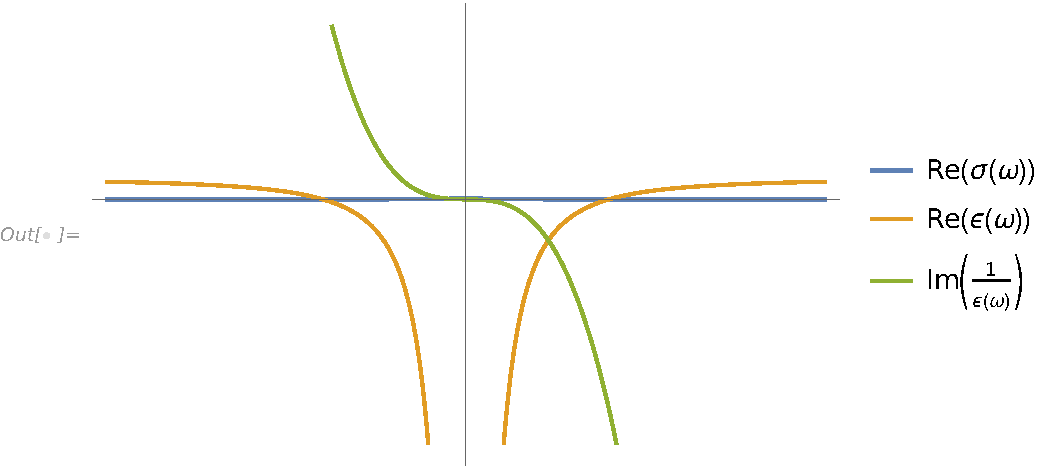
\includegraphics[width=0.6\textwidth,trim=1.5cm 0 0 0,clip]{3a}
		\caption{Plots of $\Re[\sigomg]$~(blue), $\Re[\epsomg]$~(gold), and $\Im[1 / \epsomg]$~(green).  These expressions are given by Eqs.~\refeq{3ai}, \refeq{3aii}, and \refeq{3aiii}, respectively.}
		\label{3a}
	\end{figure}
}



\prob{
	Consider a light wave with the electric field polarized in the $x$ direction at normal incidence from the vacuum on a good Drude metal occupying the region $z > 0$.  In the vacuum ($z < 0$), the incident $\Eq$ and reflected $\Ew$ waves give rise to a field
	\eq{
		\Ex = \Eq e^{i \omg (z / c - t)} + \Ew e^{-i \omg (z / c + t)},
	}
	whereas in the medium, the electric field is
	\eq{
		\Ex = \Eo e^{i \omg [ \Nomg z / c - t ]}.
	}
	Matching the electric and magnetic fields on the boundary, show that
	\al{
		\Eo &= \Eq + \Ew, &
		N \Eo &= \Eq - \Ew,
	}
	and hence show that the reflection coefficient satisfies
	\eqn{R}{
		R = \abs{\frac{\Ew}{\Eq}}^2
		= \abs{\frac{1 - N}{1 + N}}^2.
	}
}

\sol{
	By (5.15) of the lecture notes, the boundary condition is
	\eq{
		\epspar \Epar - \Dpar,
	}
	where $\epspar$ is given by Eq.~\refeq{eps}.  In this problem the surface of the metal is the $xy$ plane.  We require
	\eq{
		\Eq e^{i \omg (z / c - t)} + \Ew e^{-i \omg (z / c + t)} = \epsomg \Eo e^{i \omg [ \Nomg z / c - t ]}.
	}
	First making the ansatz $\Eo = \Eq + \Ew$,
	\al{
		\Eq e^{i \omg (z / c - t)} + \Ew e^{-i \omg (z / c + t)} &= \epsomg (\Eq + \Ew) e^{i \omg [ \Nomg z / c - t ]} \\
		\Eq [ e^{i \omg (z / c - t)} - \epsomg e^{i \omg [ \Nomg z / c - t ]} ] &= -\Ew [ e^{-i \omg (z / c + t)} - \epsomg e^{i \omg [ \Nomg z / c - t ]} ] \\
		\Eq [ e^{-2 i \omg z / c} - \epsomg e^{i \omg z [ \Nomg + 1 ] / c} ] &= -\Ew [ 1  - \epsomg e^{i \omg z [ \Nomg + 1 ] / c} ] \\
	}
	
	\hl{??????}
}



\prob{
	Using the Drude formula above, show that
	\eq{
		R \approx \begin{cases}
			1 - 2 \sqrt{\dfrac{\omg}{2\pi \sigo}} & \omg \ll 1 / \tau, \\[3ex]
			1 - \dfrac{2}{\omgp \tau} & 1 / \tau \ll \omg \ll \omgp, \\[3ex]
			0 & \omgp \ll \omg,
		\end{cases}
	}
	and sketch the reflectivity $\Romg$.
}

\sol{
	From Eq.~\refeq{R}, we can write
	\al{
		R &= \abs{\frac{1 - N}{1 + N}}^2 \\
		&= \frac{(1 - \Re[N])^2 + \Im[N]^2}{(1 + \Re[N])^2 + \Im[N]^2} \\
		&= \frac{(1 - \sqrt{\Re[\epsomg]})^2 + \sqrt{\Im[\epsomg]}^2}{(1 + \sqrt{\Re[\epsomg]})^2 + \sqrt{\Im[\epsomg]}^2} \\
		&= \frac{1 - 2 \sqrt{\Re[\epsomg]} + \Re[\epsomg] + \Im[\epsomg]}{1 + 2 \sqrt{\Re[\epsomg]} + \Re[\epsomg] + \Im[\epsomg]},
	}
	where we have used Ashcroft \& Mermin~(K.6).  Feeding in Eqs.~\refeq{3aii} and \refeq{3ax},
	\eq{
		R = \paren{ 2 - 2 \sqrt{1 - \frac{\omgp^2}{1 / \tau^2 + \omg^2}} - \omgp^2 \frac{1 + 1 / \tau \omg}{1 / \tau^2 + \omg^2} } \paren{ 2 + 2 \sqrt{1 - \frac{\omgp^2}{1 / \tau^2 + \omg^2}} - \omgp^2 \frac{1 + 1 / \tau \omg}{1 / \tau^2 + \omg^2} }^{-1}.
	}
	When $\omg \ll 1 / \tau$, $\tau \omg \ll 1$.  Then
	\al{
		R &= \paren{ 2 - 2 \sqrt{1 - \frac{\omgp^2 / \omg^2}{1 / \tau^2 \omg^2 + 1}} - \frac{\omgp^2}{\omg} \frac{1 / \omg + 1 / \tau \omg}{1 / \tau^2 \omg^2 + 1} } \paren{ 2 + 2 \sqrt{1 - \frac{\omgp^2 / \omg^2}{1 / \tau^2 \omg^2 + 1}} - \frac{\omgp^2}{\omg} \frac{1 / \omg + 1 / \tau \omg}{1 / \tau^2 \omg^2 + 1} }^{-1} \\
		&\approx \frac{ 2 - 2 \sqrt{1 - (\tau \omg)^2 \omgp^2 / \omg^2} - (\tau \omg)^2 \omgp^2 (1 + 1 / \tau) / \omg^2 }{ 2 + 2 \sqrt{1 - (\tau \omg)^2 \omgp^2 / \omg^2} - (\tau \omg)^2 \omgp^2 (1 + 1 / \tau) / \omg^2 } \\
		&\approx \frac{ [ \omgp^2 / \omg^2 - \omgp^2 (1 + 1 / \tau) / \omg^2 ] (\tau \omg)^2 }{ 4 - [ \omgp^2 / \omg^2 + \omgp^2 (1 + 1 / \tau) / \omg^2 ] (\tau \omg)^2 } \\
		&= \frac{ (\omgp^2 / \tau \omg^2) (\tau \omg)^2 }{ 4 - [ \omgp^2 / \omg^2 + \omgp^2 (1 + 1 / \tau) / \omg^2 ] (\tau \omg)^2 }
	}
	\hl{???}
	From (5.27) in the lecture notes,
	\eq{
		\sigo = \frac{\omgp^2 \tau}{4\pi}.
	}
	\eq{
		1 - 2 \sqrt{\frac{\omg}{2 \pi \sigo}} = 1 - 2 \sqrt{\frac{2 \omg}{\omgp^2 \tau}}
	}
	
	When $\omg \ll \omgp$ and $1 / \tau \ll \omg$, $\omgp / \omg \gg 1$ and $\tau \omg \gg 1$:
	\al{
		R &= \paren{ 2 - 2 \sqrt{1 - \frac{\omgp^2 / \omg^2}{1 / \tau^2 \omg^2 + 1}} - \frac{\omgp^2}{\omg^2} \frac{1 + 1 / \tau}{1 / \tau^2 \omg^2 + 1} } \paren{ 2 + 2 \sqrt{1 - \frac{\omgp^2 / \omg^2}{1 / \tau^2 \omg^2 + 1}} - \frac{\omgp^2}{\omg^2} \frac{1 + 1 / \tau}{1 / \tau^2 \omg^2 + 1} }^{-1} \\
		&\approx \frac{ 2 - 2 \omgp/ \omg - \omgp^2/ \omg^2 }{ 2 + 2 \omgp/ \omg - \omgp^2/ \omg^2 }
	}
	\hl{idek}
	
	When $\omgp \ll \omg$, $\omgp / \omg \ll 1$:
	\al{
		R &= \paren{ 2 - 2 \sqrt{1 - \frac{\omgp^2 / \omg^2}{1 / \tau^2 \omg^2 + 1}} - \frac{\omgp^2}{\omg^2} \frac{\omg^2 + \omg / \tau}{1 / \tau^2 + \omg^2} } \paren{ 2 + 2 \sqrt{1 - \frac{\omgp^2 / \omg^2}{1 / \tau^2 \omg^2 + 1}} - \frac{\omgp^2}{\omg^2} \frac{\omg^2 + \omg / \tau}{1 / \tau^2 + \omg^2} }^{-1} \\
		&\approx \frac{2 - 2 \sqrt{1}}{2 + 2 \sqrt{1}} \\
		&= \ans{ 0 },
	}
	as desired. \qed
}





\clearpage
\state{Phonons}{
	From Eq.~(5.8) construct $\Im[\chi]$ in the limit that $\gam \to 0$.  Use the Kramers--{\Kronig} relation to then reconstruct $\Re[\chi]$ from $\Im[\chi]$ in the same limit.
}

\sol{
	Equation~(5.8) in the lecture notes is
	\eq{
		\chivqomg = \frac{1}{-\rho \omg^2 + i \gam \omg + K q^2}.
	}
	Then
	\eq{
		\Im[\chi] = -\frac{\gam \omg}{(K q^2 - \rho \omg)^2 + \gam^2 \omg^2}.
	}
	In the limit $\gam \to 0$,
	\eq{
		\Im[\chi] = -\frac{\gam \omg}{(K q^2 - \rho \omg^2)^2}.
	}
	The relevant Kramers--{\Kronig} relation is given by (5.39),
	\eq{
		\Re[\kapomg] = \PrV \int \ddomgpf \frac{\Im[\kapomgp]}{\omg' - \omg}.
	}
	Then
	\eq{
		\Re[\kapomg] = -\PrV \int \ddomgpf \frac{1}{\omg' - \omg} \frac{\gam \omg'}{(K q^2 - \rho {\omg'}^2)^2}
		= 
	}
	\hl{partial fraction decomposition???}
}





%\clearpage
%\state{Screened Coulomb interaction}{
%	Consider a nucleus of charge $Z$ producing a potential
%	\eq{
%		\Vextvq = -\frac{4\pi Z e^2}{q^2}.
%	}
%	Using the long-wavelength limit of the dielectric function, show that the screened potential satisfies
%	\eq{
%		\Vscrvqo = -\frac{2}{3} \Omg \EF,
%	}
%	where $\Omg$ is the volume of the unit cell and $\EF$ is the Fermi energy for $Z$ free electrons per unit cell.
%}






%\state{Peierls transition}{
%	By rewriting the term containing $\nkpq$ (replace $\vk + \vq \to -\vk'$ and then relabel $\vk'$ as $\vk$), show that the static density response function can be written
%	\eq{
%		\chiovqo = 2 \sumklkF \frac{1}{\epskpq - \epsk}.
%	}
%	In one dimension, make a linear approximation to the electronic dispersion near $\kF$, i.e.~$\epsk = \vF \abs{k}$, and consider the response for $q = 2 \kF + p$, where $p \ll 2 \kF$.  By considering terms in the sum over $k$ near $k \approx -\kF$, show that
%	\eq{
%		\chio(2 \kF + p) \approx \frac{1}{2\pi \vF} \ln\abs{ \frac{\kF}{p} }.
%	}
%	Explain why this result suggests that a one-dimensional metal will be unstable to a lattice distortion with wavevector $2 \kF$.
%}






%\state{Optical properties}{
%	Discuss why, at optical frequencies, glass is transparent and silver is shiny, while graphite appears black and powdered sugar is white.
%}





%\state{Metals and insulators}{
%	Explain the differences between a metal and an insulator.  Your discussion should include reference to single particle properties, screening of the Coulomb interaction, optical properties, and electrical and thermal properties.
%}


\makebib

\end{document}
